% Document class options:
% =======================
%
% lineno: Adds line numbers.
%
% serif: Sets the body font to be serif. 
%
% twocolumn: Sets the body text in two-column layout. 
% 
%
% Using other bibliography styles:
% =======================
% Not supported at the moment
\documentclass[twocolumn, serif, authordate, empirical]{jote-article}


%%% Add the bibliography, make sure it's in the same directory
\addbibresource{traxler.bib}

%%% Add additional packages here if required. Usually not needed, except when doing things with figures and tables, god help you then

% This package is for generating Lorem Ipsum, usage: \lipsum[X] where X is the Xth paragraph of lorem ipsum. OR use [1-5] to generate the first five, etc.
\usepackage{lipsum}
\usepackage{enumitem}% http://ctan.org/pkg/enumitem
\setlist[itemize]{noitemsep, topsep=0pt, labelindent=\parindent, leftmargin=2\parindent, label=$\triangleright$}
\setlist[description]{noitemsep, topsep=0pt}
\setlist[enumerate]{noitemsep, topsep=0pt}


% Fill in the type of article here. Doesn't matter if capitalized. 
%%% Options
% Empirical
% Reflection
% Meta-Research
% Rejected Grant Application
% Editorial

%%% TODO: Make this a 1-5 option scale to reduce the chance of mistyping
\papertype{Empirical}

% Enter the title, in Title Case Please
% Try to keep it under 3 lines
\title{Trial and Error (-Related Negativity):\text{ }\hspace{\textwidth} An Odyssey of Integrating Different Experimental Paradigms}

% List abbreviations here, if any. Please note that it is preferred that abbreviations be defined at the first instance they appear in the text, rather than creating an abbreviations list.
%\abbrevs{ABC, a black cat; DEF, doesn't ever fret; GHI, goes home immediately.}

% Include full author names and degrees, when required by the journal.
% Use the \authfn to add symbols for additional footnotes and present addresses, if any. Usually start with 1 for notes about author contributions; then continuing with 2 etc if any author has a different present address.
\author[1,2\authfn{2}]{Juliane Traxler}
%Fill it in again for the PDF metadata. Lame workaround but it works
\authorone{Traxler, J.}

\author[1\authfn{2}]{Roxane V. Philips}
\authortwo{Philips, R. V.}
\author[1]{Andreas von Leupoldt}
\authorthree{von Leupoldt, A.}
\author[1,2]{\hspace{\textwidth}Johan W. S. Vlaeyen}
\authorfour{Vlaeyen, J. W. S.}
%List the contribution effort here, they will be listed at the end of the page
%\contributions{Equally contributing authors.}
\contributions{Equally contributing authors.}

%List the acknowledgments. If there is no companion piece, this is listed below the author info
\acknowledgments{The authors wish to thank Mathijs Franssen and Jeroen Clarysse for the brainstorming and their technical support in programming the experiment. Furthermore, the authors would like to extend their gratitude and acknowledgements to all study participants for their time and critical reflections.}
%List possible conflict of interest. Will default to saying no conflict exists.
\funding{This work was supported by the `Asthenes' long-term structural funding Methusalem grant (METH/15/011) from the Flemish Government, Belgium, and by an infrastructure grant from the Herculesstichting, Belgium (AKUL/13/07).}

% Include full affiliation details for all authors
\affil[1]{Research Group Health Psychology, KU Leuven, Leuven, Belgium}
\affil[2]{Experimental Health Psychology, Maastricht University, Maastricht, The Netherlands}

% List the correspondence email of the main correspondent
\corraddress{Juliane Traxler, Research Group Health Psychology, University of Leuven, Tiensestraat 102, Box 3726, 3000 Leuven, Belgium}
\corremail{\href{mailto:juliane.traxler@kuleuven.be}{juliane.traxler@kuleuven.be}}

% Optionally list the present address of one of the authors
%\presentadd[\authfn{2}]{Department, Institution, City, State or Province, Postal Code, Country}

% Fill in the DOI of the paper

% Always starts with "10.36850/" and is suffixed with one of the following plus a number
% e  : empirical
% r  : reflection
% mr : meta-research
% rga: rejected grant application
% ed : editorial
\paperdoi{10.36850/e2}

% Include the name of the author that should appear in the running header
\runningauthor{Traxler et al.}

% The name of the Journal
\jname{Journal of Trial and Error}

% The year that the article is published
\jyear{2020}

%The Volume Number
\jvolume{1}

\jissue{1}
\jpages{27-38}

%The website that's listed in the bottom right
\jwebsite{https://www.jtrialerror.com}

%%% Only \paperpublished is necessary, any combination of the other two is possible

%When the paper was received
\paperreceived{21 July, 2020}
% When the paper was accepted
\paperaccepted{28 November, 2020}
% When the paper will be published
\paperpublished{2 December, 2020}
% When the paper is published but in YYYY-MM-DD format, for the crossmark button
\paperpublisheddate{2020-12-2}

% The pages of the article, comment out if rolling article
%\jpages{1-12}
% Link to the logo, might be redundant
\jlogo{media/jote_logo_full.png}

% Fill something here if this is a rolling/online first article, will make ROLLING ARTICLE show up on the first page
%\rolling{YES}

% Sets the paragraph skip to be zero, this should be in the CLS
\setlength{\parskip}{0pt}

%%% Companion Piece

% Reflection and Empirical articles have each other as companion pieces. Add the DOI, Title, and Abstract of the respective Companion piece here
\companionurl{https://doi.org/10.36850/r2}
\companiontitle{Derksen (2020)}
\companionabstract{`Trial and Error (-related negativity)' is a fascinating paper detailing the attempt to develop a new experimental paradigm to study the role of error-related negativity in the development of avoidance behavior. In my comments on this paper I will focus on the interaction between experimenters and participants as the former investigate various ways of designing the experiment, aiming to elicit the right kind of behavior from the participants. As in many psychological experiments, there is a fundamental tension here that experimenters must find a way to deal with: they must guide the subject to the proper performance, without the subject responding to the guidance as such. The performance must be natural, but within tight constraints. Recalcitrance or resistance of the subject must be prevented. Ultimately, the authors of ‘Trial and Error (-related negativity)’ failed in their attempt to do this. Their reflections on their failure are thorough and illuminating, but I will argue that they can be pushed slightly further.}
\companionkey{Derksen2020}
%%% Abstract

% These two set the height and width of the abstract. There's no solution to do this automatically at the moment so fiddle with these a bit. height-width should be 5mm, and ranges between 50-100 are realistic
% Higher number means skinnier abstract
\heightabstract{48mm}
\widthaffil{43mm}
%Enter something here in order for the abstract to disappear. Be sure to also delete the abstract 
\noabstract{}
% Fill in the keywords that will appear in the abstract, max 7
\keywordsabstract{error-related negativity, avoidance behavior, chronic pain, experimental psychopathology, experimental paradigm}

%%%%%%%%%%%%%%%%%%%%%%%%%%%%%%%%%%%%%%%%%%%%%%%%%%%
%Document Starts
%%%%%%%%%%%%%%%%%%%%%%%%%%%%%%%%%%%%%%%%%%%%%%%%%%%

\begin{document}
%%% This starts the frontmatter, which includes everything that's on the front page execpt the text of the article
\begin{frontmatter}
\pdfbookmark[0]{Traxler, J. et al. - Trial and Error (-Related Negativity):An Odyssey of Integrating Different Experimental Paradigms}{traxlerpdf}
\maketitle
%Type your abstract between these things. Max 250 words. Be sure to include the \noindent, looks bad otherwise
\begin{abstract}
    Pain can be considered as a signal of "bodily error'': Errors — discrepancies between the actual and optimal/targeted state — can put organisms in danger and activate behavioral defensive systems. If the error relates to the body, pain is the warning signal that motivates protective action such as avoidance behavior to safeguard our body's integrity. Hence, pain shares the functionality of errors. On the neural level, an important error-processing component is error-related negativity (ERN), a negative deflection in the electroencephalographic (EEG) signal generated primarily in the anterior cingulate cortex within 100 ms after error commission. Despite compelling evidence that the ERN plays an important role in the development of various psychopathologies and is implicated in learning and adjustment of behavior, its relation to pain-related avoidance has not yet been examined. Based on findings from anxiety research, it seems conceivable that individuals with elevated ERN amplitudes are more prone to engage in pain-related avoidance behavior, which may, under certain conditions, be a risk factor for developing chronic pain. Consequently, this new line of research promises to contribute to our understanding of human pain. As in most novel research areas, a first crucial step for integrating the scientific fields of ERN and pain is developing a paradigm suited to address the needs from both fields. The present manuscript presents the development and piloting of an experimental task measuring both ERN and avoidance behavior in response to painful mistakes, as well as the challenges encountered herein. A total of 12 participants underwent one of six different task versions. We describe in detail each of these versions, including their results, shortcomings, our solutions, and subsequent steps. Finally, we provide some advice for researchers aiming at developing novel paradigms.
\end{abstract}
\end{frontmatter}
\setcounter{page}{27}

%% Purpose


\phantomsection \addcontentsline{toc}{section}{Take-home message}\section*{Take-home message} 

Developing a new experimental paradigm is challenging, time-consuming and requires thorough testing. To improve the efficiency of this process, we advise to clearly define the requirements at the beginning, to keep record of all decisions and adjustments made in the process, and to investigate encountered problems and failures which may help to gradually improve the paradigm.


\phantomsection \addcontentsline{toc}{section}{Purpose}\section*{Purpose} 

Avoidance behavior is part of a natural defense mechanism that is activated when individuals are experiencing chronic pain. In order to shed more light on the neural underpinnings of pain avoidance behavior, our long-term aim is to investigate its association with the error-related negativity (ERN), an important component of neural error processing. So far, the ERN has been predominantly examined in relation to anxiety disorders and has been suggested as an endophenotype of obsessive-compulsive disorder \parencite{Riesel2011}. Initially, ERN research focused on its relationship with the tendency to learn best from negative feedback \parencite{Frank2005}, whereas a few more recent studies also observed greater disorder-specific defensive motivation and avoidance behavior in individuals with elevated ERN amplitudes \parencite{Riesel2019, Riesel2019b, Weinberg2016}. These findings support the assumption that the ERN may be similarly implicated in pain-related avoidance, but this possibility remains to be tested.~Investigating this theoretically plausible association may improve our general understanding of the neural mechanisms underlying avoidance behavior and help to identify individuals at risk of developing chronic pain.~The novelty of this endeavor requires the integration of knowledge of both research strands, as well as the development of an experimental paradigm that is well-suited to their respective requirements. Here, we describe the process of developing and piloting such a paradigm and provide an overview of problems encountered herein. We conclude with a tutorial section on the development of novel experimental paradigms based on our experience with this specific study, which we hope is also broadly applicable.


\phantomsection \addcontentsline{toc}{section}{Introduction}\section*{Introduction} 

Chronic pain affects as many as 20\% of adults in Europe \parencite{SocietalImpactofPain2017}. This poses a considerable healthcare challenge and causes tremendous individual suffering. Many chronic pain conditions are best understood from a biopsychosocial perspective which acknowledges the complex interplay of organic, cognitive, emotional, behavioral, and social factors. For example, on the neurobiological level, the sensitization model states that following acute pain, hypersensitization of local nerves occurs, causing exaggerated pain perception, or a lowered pain threshold, which may initiate a spiral in which hypersensitization triggers pain, which in turn triggers sensitization \parencite{vanWilgen2012, Meeus2007}. Although the sensitization model is very intuitive, and often used as a metaphor in pain education with patients, it has also been criticized (e.g., \nptextcite{vandenBroeke2019}). On the cognitive and behavioral level, one of the most prevalent explanations for the transition from a common acute pain episode to chronic disabling pain is the fear-avoidance model \parencite{Vlaeyen2016, Vlaeyen2000, Vlaeyen2020}. It posits that pain-related avoidance behavior, often fueled by catastrophic (mis)interpretations of pain, contributes to individuals entering a downward spiral of fear, avoidance, inactivity, disability, and negative affect. Pain avoidance refers to individuals avoiding stimuli that are predictive of pain or pain exacerbations. For instance, persons who have sustained an injury to their back may avoid lifting objects for fear that it will lead to further pain, or that lifting may create bodily harm that is signaled by pain. Typically, avoidance occurs in anticipation of pain, and hence individuals have little opportunity to test and, if necessary, correct their beliefs about the threat associated with such activities. This failure to correct mistaken beliefs maintains pain-related fear and further increases mood disturbances and pain itself \parencite{vanVliet2018, Vlaeyen2000}.~

The neural underpinnings of pain-related avoidance behavior are poorly understood. A new and promising avenue to understanding pain-related avoidance is to study its relation to error-related negativity (ERN). The ERN is an event-related potential (ERP), which occurs within \textasciitilde100 ms after error commission \parencite{Hajcak2012}. It can be measured as a negative deflection in the electroencephalogram (EEG) over fronto-central scalp positions, originating in the anterior cingulate cortex \parencite{Falkenstein2000, Gehring1993, Miltner2003, Taylor2007}. Differences in the amplitude of the ERN are affected by both contextual and individual factors such as motivational aspects and error salience, and are considered to reflect individual error sensitivity \parencite{Hajcak2012, Hajcak2008, Taylor2007}. For instance, it has been observed that the ERN is larger when errors are perceived to have worse consequences \parencite{Hajcak2012}. Additionally, the ERN is believed to activate a defensive motivational system in order to adjust the erroneous behavior and protect the organism \parencite{Hajcak2008}. In line with these findings, increased ERN amplitudes have consistently been associated with anxiety disorders \parencite{Weinberg2012, Hanna2020} as persons affected arguably perceive their own mistakes in relation to the respective object of fear as highly threatening.~In addition, avoidance behavior (including experiential avoidance) is a typical feature of anxiety disorders \parencite{Aupperle2010, Berman2010, Dikman2000, Dymond2009}.

Given the commonalities between anxiety disorders and chronic pain \parencite{Asmundson2009}, and the high prevalence of negative affect in chronic pain \parencite{Geisser2000}, it is theoretically plausible that the ERN\footnote{Readers familiar with the error processing literature may wonder why we do not consider the Pe (error positivity), a later component of neural error processing. The reason is that we have no particular   hypotheses about its relationship with pain-related avoidance, as it has not been as extensively studied in anxiety research as the ERN, especially with regard to avoidance behavior. We do aim to explore it in upcoming studies, but our main target of this report is the ERN, therefore we focused on developing a paradigm suitable to measure the ERN.} may be a biomarker for the development of pain-related avoidance behavior as well. In the case of anxiety, the particular feared object is considered threatening, whereas individuals with chronic pain perceive pain to be highly threatening. Because pain is such a salient and aversive stimulus, which conceptually signals bodily error and is often interpreted as such, avoidance responses constitute a defense mechanism to prevent the feared outcome \parencite{Leeuw2007}. As such we may see an association between the ERN amplitude and the level of avoidance exhibited by an individual, with avoidance representing a defensive behavior in response to a motivationally salient and aversive stimulus.~

Our long-term goal is to investigate whether individual differences in the ERN amplitude are related to differences in pain-related avoidance behavior, which may help identify individuals more at risk for the development of chronic disabling pain. To this end, we aimed to create an experimental paradigm that would allow us to measure the ERN and avoidance responses simultaneously, the process of which is described in the present manuscript. Previous experiments that studied this relationship in our lab (Traxler et al., in preparation) used the visual Flanker task unrelated to pain and had participants coming in on a separate day to measure pain avoidance behavior using a robotic arm (HapticMaster). A task integrating both the ERN and pain avoidance seems more efficient than measuring them in separate tasks. It also ensures that there is a relation between error commissions and pain-related avoidance, as it is for instance not clear how inhibition errors on a visual task relate to pain-related avoidance. Additionally, it puts less burden on the participant. Such a paradigm would need to meet requirements for both measures (ERN and pain-related avoidance), namely: (1) evoke an ERN; (2) yield a reliable estimate of the ERN, requiring a minimum of six errors \parencite{Olvet2009, Steele2016}; and (3) be able to detect individual differences in avoidance behavior by providing sufficient opportunities to avoid (at least 20)\footnote{This is a somewhat arbitrary criterion reflecting the problem that too   few error trials leave only little room for observing individual   differences in avoidance. In the absence of empirical data regarding   such a criterion, we based our decision on recent avoidance studies in   our and others' labs that used acquisition phases of avoidance that   usually consisted of around 20 trials. This makes it possible to   detect avoidance patterns across participants \parencite{Meulders2016, Vervliet2015}.}. Although there is some debate as to whether one needs to be aware of having committed an error to evoke the ERN \parencite{Nieuwenhuis2001}, awareness is essential in this task as participants would otherwise be unable to perform the avoidance response. In addition, the task ought to evoke inhibition errors rather than errors due to lack of skill or knowledge. For that purpose, we decided to integrate two experimental tasks, one of which is frequently used to measure the ERN (the Eriksen Flanker task; \nptextcite{Eriksen1974}) and the other is a common assessment of avoidance behavior (the avoidance task by \nptextcite{Vervliet2015}). We piloted this basic paradigm and continuously adjusted it based on the pilot results, leading to a total of six task variations. The present article focuses on the design and execution of these different tasks, what we can learn from them, and on suggestions for future research.~


\phantomsection \addcontentsline{toc}{section}{Methods}\section*{Methods}  

\phantomsection \addcontentsline{toc}{subsection}{Participants} \subsection*{Participants}

Twelve participants (8 females) took part in the pilot study between January and March of 2020. They were recruited by word of mouth, had a mean age of M = 29.25 (SD = 10.64), and gave autonomous consent. The exclusion criteria were self-reported: (a) pregnancy, (b) diagnosis of a psychiatric disorder (e.g. depression, anxiety, etc.), (c) a serious medical illness (e.g. diabetes mellitus, cardiovascular disease, neurological problems, etc.), (d) skin disease or condition where electrocutaneous stimuli could cause damage (e.g. an operation scar at the site where the electrodes would be placed), (e) pain: acute (e.g. due to an injury) or chronic, (f) electronic implant (e.g. pacemaker), (g) having been asked by a doctor to avoid stressful situations, and (h) poor vision or hearing that is not corrected. Participants gave written informed consent at the onset of the experimental session. Participants did not receive compensation for participation and mostly consisted of colleagues and acquaintances who were blinded with respect to the main aim of the tasks. The procedures conformed to the Helsinki Declaration and were approved by the institutional ethics committee (Social and Societal Ethics Committee; approval reference number: G-2019 12 1905).~


\phantomsection \addcontentsline{toc}{subsection}{Apparatus}\subsection*{Apparatus}  

\phantomsection \addcontentsline{toc}{subsubsection}{Electroencephalography} \subsubsection*{Electroencephalography} Event-related potentials in response to errors and correct trials were measured by means of electroencephalography (EEG) which was continuously recorded from the scalp using a 129-channel system (HydroCel Geodesic Sensor Net, Philips Electrical Geodesics Inc., Eugene, USA). The sampling rate was set at 250 Hz \parencite{Trujillo2007, Hajcak2005, Hajcak2008}, electrode impedances were kept below 50 kΩ and the vertex electrode was used as reference point \parencite{Sucec2019, Tan2019}.

\phantomsection \addcontentsline{toc}{subsubsection}{Stimulation} \subsubsection*{Stimulation} Vibrotactile stimuli were administered to the left side of participants' lower back through two vibrotactors (Dancer Design, St Helens, England) placed 2 cm apart (center to center; Figure \ref{fig:1}). The stimulus duration was 112 ms and the vibration intensity, which was set to a clearly perceptible level that remained non-painful throughout the experiment, was kept constant across participants. Tactors were activated in a semi-randomized order.

Electrocutaneous stimuli (e-stim) were generated by a constant-current stimulator (DS7A; Digitimer, Welwyn Garden City, England) and delivered for a duration of 2 ms through two 4 mm Ag/AgCl reusable snap electrodes filled with K-Y gel attached 1 cm above the vibrotactors. The intensity of these stimuli was individually calibrated to a level that was "painful and demanding some effort to tolerate''. For that purpose, a series of stimuli of ascending intensity was administered, each of which participants were instructed to verbally rate on a scale ranging from 0 (no sensation) to 10 (worst imaginable pain). The calibrated stimulus intensity was kept constant throughout the task.

The lower back was selected as stimulus location for two reasons: (1) the sensory acuity at the back is relatively low compared to more typical distal stimulation sites, such as the arms or hands \parencite{Weissman-Fogel2012}, which was considered advantageous with regard to task difficulty; and (2) a large, even surface area was required to attach the vibrotactors and electrodes.

\phantomsection \addcontentsline{toc}{subsubsection}{Software}\subsubsection*{Software} The experimental task was programmed and presented in Affect 5 \parencite{Spruyt2009a}, which was run on a Windows 7 Professional (Microsoft Corporation Redmond) 64 bit Dell OptiPlex 780 (Dell Inc, Round Rock, TX) with 4-GB RAM, Duo-CPU at 3.10 GHz.


\phantomsection \addcontentsline{toc}{subsection}{Measures}\subsection*{Measures} 

The purpose of the pilot study was to create a task that allows to measure the ERN and avoidance behavior simultaneously. In each task version vibrotactors emitted vibrations on participants' left lower back, EEG in response to correct and error trials was recorded, and painful e-stim were applied when participants made an erroneous response which they could omit by pressing the space bar. Avoidance was operationalized as the number of button presses to cancel an e-stim.

After performing the task participants were asked open questions to receive their perspective of the task and to ensure that requirements were met. Specifically, they were asked whether they were able to perceive when they made errors, how difficult they found the task as well as initiating the avoidance response, and any additional comments they would like to provide.

\phantomsection \addcontentsline{toc}{subsection}{General procedure}\subsection*{General procedure} 

All task versions were based on a tactile task that was inspired by Eriksen's Flanker task \parencite{Eriksen1974} and a fear-avoidance paradigm established by \textcite{Vervliet2015}. The Eriksen Flanker task typically consists of presentations of arrow stimuli, (e.g. \textless\textless{} \textgreater{} \textless\textless), and participants are asked to indicate the direction in which the center arrow points by pressing one of two buttons as quickly as possible. The flanker arrows can be congruent or incongruent and thus potentially cause inhibition errors\footnote{  We seek to elicit inhibition errors, as this is how the ERN is traditionally measured \parencite{Ribes-Guardiola2020} with participants being aware of having committed such an error.
}. In Vervliet \& Indekeu's avoidance task, participants view an office space on a monitor, in which a desk lamp can take one of three colors. Each color is indicative of whether or not an e-stim will be delivered. Participants may press a button to avoid the e-stim and learn to avoid based on the color of the lamp.

In the tactile task participants were instructed to distinguish between locations of vibrations emitted on their left lower back. We opted for tactile stimuli because these stimuli are more relevant and ecologically valid for pain responses, and more strongly resemble the tactile and proprioceptive input that frequently precedes or co-occurs with pain. Much like the arrow version of the Eriksen Flanker task in which the direction of arrows is the cue for a correct response, participants used left and right mouse buttons to indicate whether they felt a vibration at the left or right location respectively. Participants were instructed to respond as quickly and as accurate as possible. In addition, participants were informed that upon error commission they would receive an electrocutaneous stimulus, which they could cancel by pressing the space bar on the keyboard. This discrimination task was used in all task versions. Tasks employed either two or three vibrotactors (Figure \ref{fig:1}). The left and right tactors will be referred to as "target tactors'', as they emit the target stimuli that are to be discriminated by the participant. The third tactor is referred to as the "distractor tactor'' as it is meant to make the discrimination task more difficult.

\begin{figure}
    \centering
    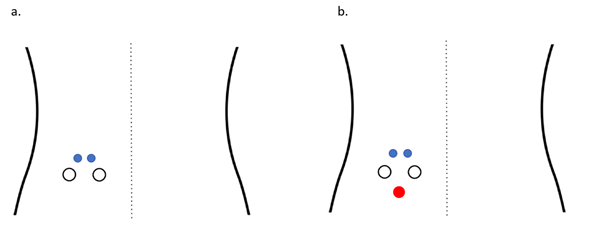
\includegraphics[width=\columnwidth]{articles/empirical/traxler/Figure 1_Trial and Error (-Related Negativity) (5).png}
    \caption{Electrode and tactor placements, with electrodes in blue. (a) Two tactor placement. (b) Three tactor placement with the red tactor indicating the distractor tactor.}
    \label{fig:1}
\end{figure}

A typical trial proceeded as follows (see Figure \ref{fig:2}): A vibration was emitted (112ms), followed by a response window, to indicate the location of the vibration (200-1000ms)\footnote{Non-responses or late responses did not bear any consequences as other studies conducted in our lab showed that participants do not simply cease to respond, even if this could be an alternative way of avoiding the painful stimulation.
}. After a fixation period (300 ms), participants could provide an avoidance response (1000 ms). If participants chose not to avoid the e-stim upon error commissioning, an e-stim was delivered following this response window. The trial concluded in a jittered intertrial interval (600-1000 ms). To prevent "better safe than sorry" reasoning for performing the avoidance response and to mimic the costs that real-life avoidance typically bears, participants were told that five, and later two, trials would be added to the duration of the experiment every time they cancelled an e-stim. In reality no trials were added. As this proved to be highly aversive to the participants, leading to an unwillingness to avoid, we removed this clause after the eighth participant. The base settings for the tasks are as follows: vibrations are set to the same intensity and the third (distractor) tactor coactivates with every target stimulation. Task versions replace one another rather than being superimposed. Any deviations from the general procedure will be indicated, with Table \ref{tab:1} giving an overview of the task versions. In general, the task versions were composed of four or five blocks of 60 trials each, Table \ref{tab:2} indicates the total number of participants and trials per task version. In total, six different versions of the task were tested: \emph{Two Tactor task}, \emph{Distractor task}, \emph{100\% coactivation task}, \emph{Different intensities task}, \emph{50\% coactivation task}, and a \emph{Sequence task}.

\begin{figure}
    \centering
    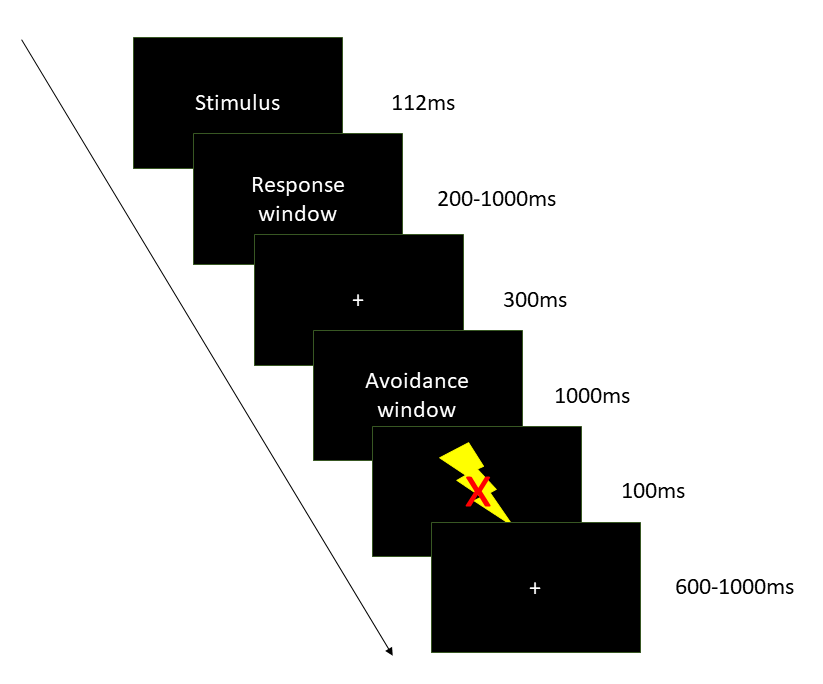
\includegraphics[width=\columnwidth]{articles/empirical/traxler/Figure 2_Trial and Error (-Related Negativity) (5).png}
    \caption{Schematic representation of the basic trial flow with exact timings depending on the task version.}
    \label{fig:2}
\end{figure}


\begin{table*}\sffamily
\begin{tabular}{@{}p{0.17\textwidth}p{0.12\textwidth}p{0.17\textwidth}p{0.12\textwidth}p{0.3\textwidth}}
\toprule Task & Number of Tactors & Stimulation intensity & Number of tasks & When does the distractor tactor activate?\tabularnewline \midrule 
Two Tactor & 2 & equal & 1 & NA\tabularnewline Distractor & 3 & equal & 2 & Plays a song\tabularnewline 100\% coactivation & 3 & equal & 1 & With every target stimulus\tabularnewline Different Intensities & 3 & 3rd tactor more intense & 1 & With every target stimulus\tabularnewline 50\% Coactivation & 3 & equal & 1 & With 50\% of target stimuli\tabularnewline Sequence & 3 & equal & 1 & With every target stimulus\tabularnewline \bottomrule 
\end{tabular}
\caption{Overview of manipulations over task versions.}
\label{tab:1}
\end{table*}

\emph{Note.} Number of tasks refers to whether participants had to perform any additional tasks to the discrimination task. \emph{Tasks are listed in the order in which they were tested.}

\phantomsection \addcontentsline{toc}{subsection}{Two Tactor task}\subsection*{Two Tactor task} 
\phantomsection \addcontentsline{toc}{subsubsection}{Procedure}
\subsubsection*{Procedure}
In this first version of the task, target tactors were attached to the left lower back of the participants (Figure \ref{fig:1}, a). Participants indicated via left and right mouse button press whether they felt a vibration at the left or right location, respectively. Upon error commission participants were free to cancel the e-stim by pressing the space bar.~One participant completed four blocks of this task version.

\phantomsection \addcontentsline{toc}{subsubsection}{Evaluation}
\subsubsection*{Evaluation} After running one participant it was quickly established that this task was too easy. This was reflected by participant feedback as well as the number of errors (\emph{M}\textsubscript{\emph{error}} = 2).~The participant was aware of having made mistakes but chose not to give any avoidance responses.


\phantomsection \addcontentsline{toc}{subsection}{Distractor task}\subsection*{Distractor task} 

\phantomsection \addcontentsline{toc}{subsubsection}{Procedure}
\subsubsection*{Procedure} In order to increase task difficulty, three tactors were attached to the left lower back, with the two target tactors at their original locations and the third, the distractor tactor, placed centrally below them (Figure \ref{fig:1}, b). This distractor tactor emitted vibrations to the beat of a widely known song (e.g., ``Seven Nation Army'' by The White Stripes). Participants were still expected to perform the same discrimination task (i.e., indicate on each trial whether the left or right tactor became active). Additionally, at the end of each block they had to choose, in a multiple choice manner, which song the distractor tactor had been vibrating to.~One participant completed four blocks of 60 trials.~

\phantomsection \addcontentsline{toc}{subsubsection}{Evaluation} \subsubsection*{Evaluation} There were several issues with this task version. The task appeared to be difficult, leading the participant to be exclusively focused on the discrimination task (\emph{M}\textsubscript{\emph{error}} = 10). Additionally, even though participants wore earplugs to prevent them from distinguishing vibrations based on the sound they made, the distractor tactor acted as a small speaker, and the participant became aware of the song because they could hear it. Due to these issues we did not run any further participants on this task.


\phantomsection \addcontentsline{toc}{subsection}{100\% coactivation task} \subsection*{100\% coactivation task}

\phantomsection \addcontentsline{toc}{subsubsection}{Procedure} \subsubsection*{Procedure} This task version used three tactors. The distractor tactor emitted vibrations simultaneously with the target tactors, in an effort to make their activations harder to discriminate. The first participant for this task completed four blocks; the subsequent six participants completed five blocks of this task. By increasing the number of blocks we sought to establish whether increasing task length would lead to more consistently elevated error commissions. Consistently higher error commissions across participants would ensure that less participants are excluded from analysis, were the paradigm to be used in the future. It would also enable us to make more reliable estimates of the ERN and individual differences in avoidance responses. One participant only completed two blocks of this task as they then completed two blocks of the 50\% coactivation task. All but one participant were told that additional trials would be added if they chose to cancel the e-stim. In an attempt to balance the trade-off and increase the cost of not avoiding, the painful stimulation was made more threatening by stating that a "stimulus with a slightly higher intensity than the one previously calibrated" could be delivered occasionally for four participants in the task (this manipulation was discontinued simultaneously with the added trials' cost).

\phantomsection \addcontentsline{toc}{subsubsection}{Evaluation} \subsubsection*{Evaluation} On average 22.5 mistakes were made across eight participants. Participant feedback indicated that the task was not too difficult and that they were conscious of having committed an error as it occurred.

\phantomsection \addcontentsline{toc}{subsection}{Different intensities task}\subsection*{Different intensities task} 

\phantomsection \addcontentsline{toc}{subsubsection}{Procedure} \subsubsection*{Procedure} This task used the 100\% coactivation schedule, with the distractor tactor set to a higher intensity than the target tactors. The goal, once more, was to make the task more difficult, in an attempt to raise the number of error commissions across participants. One participant performed five blocks of this task.

\phantomsection \addcontentsline{toc}{subsubsection}{Evaluation} \subsubsection*{Evaluation} Although this task did raise the number of error commissions (\emph{M}\textsubscript{\emph{error}} = 33), according to participant feedback, the participant was less aware of having made a mistake and therefore unable to avoid the e-stim.~

\phantomsection \addcontentsline{toc}{subsection}{50\% coactivation task} \subsection*{50\% coactivation task}

\phantomsection \addcontentsline{toc}{subsubsection}{Procedure} \subsubsection*{Procedure} In this task the distractor tactor only coactivated with target tactors 50\% of the time. This adaptation was expected to make the task more difficult as participants may habituate less to the sensation of the third tactor. Two participants completed respectively two and one block on this task.

\phantomsection \addcontentsline{toc}{subsubsection}{Evaluation} \subsubsection*{Evaluation} This task proved to be easier than its 100\%
coactivation counterpart, with the two participants making 18.5 mistakes on average.~Participants reported having difficulty recognizing error commission, as such further task versions were explored.

\phantomsection \addcontentsline{toc}{subsection}{Sequence task}\subsection*{Sequence task} 

\phantomsection \addcontentsline{toc}{subsubsection}{Procedure} \subsubsection*{Procedure} In this last task, participants were instructed to recreate sequences of three vibrations using button presses. The target tactors went off in a sequence (e.g., left-right-right), and participants recreated this using the left and right mouse buttons. The distractor tactor followed a 100\% coactivation schedule, i.e., coactivated with the target vibrations on each trial. Two participants performed five blocks of the task. We expected that this task would be more difficult as it required a more speeded response from the participants. Additionally, we thought it might lead to more inhibition errors: In the arrow version of the Flanker task, incongruent trials (i.e., those in which the middle arrow points in the opposite direction of the flanking arrows) tend to evoke more errors. Similarly, on the present task, two left activations, for instance, may mislead the participant to expect another left activation, instead of a right.

\phantomsection \addcontentsline{toc}{subsubsection}{Evaluation} \subsubsection*{Evaluation} This task provided inconsistent results as the deviations in the number of error commissions varied widely between participants (pilot\textsubscript{a}: \emph{M}\textsubscript{\emph{error}} = 73, pilot\textsubscript{b}: \emph{M}\textsubscript{\emph{error}} = 12). Though individual differences in performance are to be expected in any task, the task should be reliable in evoking the needed number of error commissions. Participants were aware of their error commissions.~

\phantomsection \addcontentsline{toc}{subsection}{Statistical Analysis}\subsection*{Statistical Analysis} 

The EEG data was processed in Brain Electrical Source Analysis Research 6.0 (BESA GmbH, Gräfelfing, Germany), using a high-cut filter of 30 Hz, a low-cut filter of 0.1 Hz and a notch filter of 50 Hz \parencite{Gorka2019}. Ocular artifact removal was performed using the BESA algorithm, which does not require the measurement of an additional electrooculogram (EOG), but uses fronto-facial sensors to detect ocular movements. Bad channels were interpolated or deleted upon visual inspection, with a maximum of 12 bad channels {(}10\% of the total number of electrodes; \parencite{Keil2014}{)}. Response-locked epochs of 1500 ms (500 ms pre- and 1000 ms post-response) were extracted and averaged per participant, using the 500-300 ms pre-response interval as baseline \parencite{Jackson2015, Tan2019, Gorka2019}. Data were re-referenced to the average reference.

The ERN was operationalized as the mean amplitude in the 0 to 100 ms time window after error commission at the fronto-central site FCz (Geodesic net electrode 6) \parencite{Hajcak2019a}. In addition, the correct response negativity (CRN) — a similar yet smaller negative deflection in the EEG signal following correct responses (0-100 ms post-response) — was computed in the same way. The difference score between the ERN and the CRN, known as the $\Delta$ERN, will be reported. Previous research suggests that the validity of the $\Delta$ERN is higher than that of the mean amplitude of the ERN alone \parencite{Riesel2013, Gorka2019}. Both the preprocessed EEG and behavioral data were analyzed using R \parencite{RCoreTeam2013}. Due to the small group sizes across tasks and resulting insufficient statistical power to make reliable inferential conclusions, the analysis consists mostly of descriptive statistics.


\phantomsection \addcontentsline{toc}{section}{Results}\section*{Results} 

EEG data were recorded for 10 of the 12 participants, including both \emph{Sequence task} pilots, the \emph{Different intensities} pilot, one \emph{50\% coactivation} pilot, and six \emph{100\% coactivation}
pilots. One participant on the 100\% coactivation task committed less than six errors and was therefore excluded from the EEG analyses. No EEG data were recorded for the \emph{Distractor} task or \emph{Two Tactor}
task. Given the small sample size, the results presented below need to be read with caution and should only be evaluated with regard to the pre-specified task criteria.

\phantomsection \addcontentsline{toc}{subsection}{Task performance and avoidance behavior}\subsection*{Task performance and avoidance behavior} 

On average, participants committed 24.07 errors (\emph{SD} = 18.33, \emph{range} = 0-73, 10.59\% of all accepted responses) and gave 203.21 correct responses (\emph{SD} = 98.82, \emph{range} = 1-297) on the discrimination task. A Related Samples Wilcoxon Signed Rank Test revealed that reaction times were significantly faster during correct trials (\emph{M} = 527.35 ms, \emph{SD} = 88.39) compared to error trials (\emph{M} = 619.53 ms, \emph{SD} = 114.75; \emph{Z} = 3.059, \emph{p} = .002)\emph{.}

Table \ref{tab:2} shows the results for the behavioral responses. The \emph{Two Tactor} task yielded few mistakes (\emph{M} = 2, \emph{SD} = 0) and no avoidance responses. The \emph{100\% coactivation} task produced more error commissions (\emph{M} = 22.5, \emph{SD} = 20.61), and some avoidance responses (\emph{M} = 7.12, \emph{SD} = 16.25). The \emph{Different intensities} task version led to a higher number of mistakes (\emph{M} = 33, \emph{SD} = 0), but did not produce any avoidance responses. Moving on to the \emph{50\% coactivation} task, we observe a comparable average error commission as for the \emph{100\%
coactivation} task (\emph{M} = 18.5, \emph{SD} = 19.09). However, the frequency of avoidance is low (\emph{M} = 0.5, \emph{SD} = 0.7). This might indicate either that participants are unaware of having committed an error and thus are unable to avoid, or that they were unwilling to bear the costs introduced with this task version. The \emph{Sequence}
task produced the highest average error commissions (\emph{M} = 42.5, \emph{SD} = 43.13), but these scores are highly inconsistent across participants. The same applies to the avoidance responses in this task (\emph{M} = 27.5, \emph{SD} = 19.09). The \emph{Distractor} task shows only \emph{M} = 10 error commissions (\emph{SD} = 0) and no avoidance responses. Note that results for each task version are based on unequal and few data points (Table \ref{tab:2}).~

We further compared when the most error commissions occurred in each task, in order to determine whether mistakes are more likely to be attributable to the novelty of the task or whether the task manages to consistently evoke error commissions. Across tasks, 56\% of errors occurred in the first two blocks of the experiment. Note that for participants whose total number of trials was lower than four blocks, only the first block was considered. The task that evoked errors the most consistently throughout the blocks was the \emph{100\% coactivation} task (45.8\% of errors in the first two blocks) and the least was the \emph{Different intensities} task (81.8\% of errors in the first two blocks).~

\begingroup
\hyphenpenalty10000
\begin{table}[h]\sffamily
\begin{tabular}{@{}>{\raggedleft\arraybackslash}p{0.15\columnwidth}>{\centering\arraybackslash}b{0.005\columnwidth}>{\centering\arraybackslash}b{0.066\columnwidth}>{\centering\arraybackslash}b{0.03\columnwidth}>{\centering\arraybackslash}b{0.06\columnwidth}>{\centering\arraybackslash}b{0.08\columnwidth}>{\centering\arraybackslash}b{0.08\columnwidth}>{\centering\arraybackslash}b{0.07\columnwidth}>{\centering\arraybackslash}b{0.04\columnwidth}}
\toprule 
& & &\multicolumn{3}{c}{Errors} & & &\tabularnewline [-4ex]
Task & N & Total trials & M & SD & Range  & Mean Avoided & $\Delta$ERN & Peak (ms) \tabularnewline \midrule 
Two Tactor & 1 & 240 & 2 & 0 & 2 & 0 & NA & NA\tabularnewline 
Distractor & 1 & 240 & 10 & 0 & 10 & 0 & NA & NA\tabularnewline 100\% Coactivation & 8 & 2100 & 22.5 & 20.61 & 0-64 & 7.12 & -3.97 & 0\tabularnewline Different Intensities & 1 & 300 & 33 & 0 & 33 & 0 & -0.43 & 68\tabularnewline 50\% Coactivation & 2 & 180 & 18.5 & 19.09 & 5-32 & 0.5 & -0.02 & 28\tabularnewline Sequence & 2 & 600 & 42.5 & 43.13 & 12-73 & 27.5 & -0.05 & 52\tabularnewline \bottomrule \end{tabular}
\caption{Results of behavioral and EEG data}
\label{tab:2}
\end{table}
\endgroup
\phantomsection \addcontentsline{toc}{subsection}{Error-related negativity}\subsection*{Error-related negativity} 

Figure \ref{fig:3} shows the response-locked ERPs and topographies for error and correct responses across the four task versions (\emph{Sequence}, \emph{Different intensities}, \emph{50\% coactivation}, \emph{100\%
coactivation}) separately. All four tasks do show the potential for evoking an ERN with negative going deflections being observed at the expected fronto-central locations. Across all tasks, the average difference score between ERN and CRN was \emph{$\Delta$ERN} = -2.27µV. The task showing the most pronounced $\Delta$ERN at FCz is the \emph{100\% coactivation}
task (\emph{$\Delta$ERN}= -3.97µV) and the least pronounced $\Delta$ERN was observed in the \emph{50\% coactivation} task (\emph{$\Delta$ERN}= -0.02µV). Though $\Delta$ERN scores are variable across studies \parencite{Buzzell2017, Barker2015, Gorka2019}, our results do suggest smaller difference scores than observed using traditional reaction time tasks. Importantly, given the small sample size for each task, no comparative conclusions can be drawn with regards to the ERN and its relation to pain-related avoidance responses across tasks.~

\begin{figure*}
    \centering
    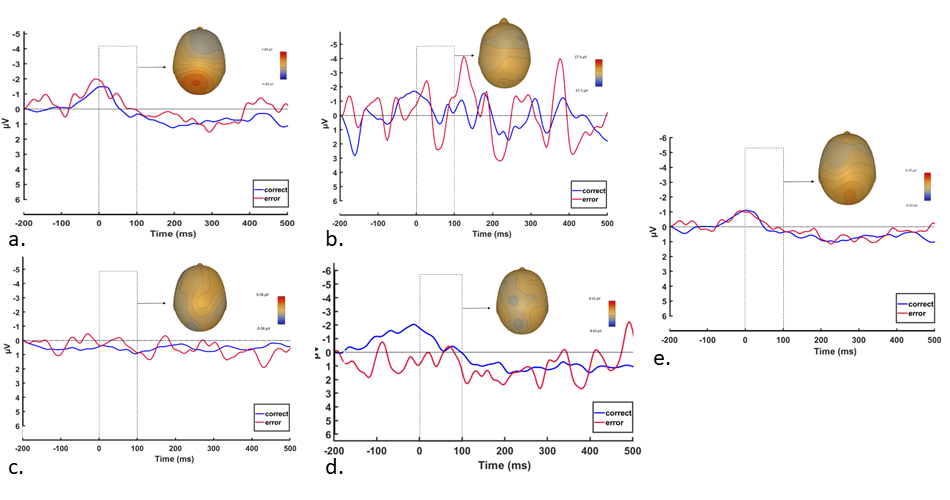
\includegraphics[width=\textwidth]{articles/empirical/traxler/figure3.png}
    \caption{Response-locked grand average waveforms for ERN and CRN at Cz with topography, averaged for (a) the \emph{100\% coactivation task} (N = 5); (b) the \emph{50\% coactivation task} (N = 2); (c) the \emph{Sequence task} (N = 1); (d) the \emph{Different intensities task}
(N = 1); and (e) averaged across the four task versions (N = 9).}
    \label{fig:3}
\end{figure*}


\phantomsection \addcontentsline{toc}{section}{Discussion}\section*{Discussion} 

Here we describe the piloting of a novel paradigm based on the integration of two experimental tasks stemming from different fields of psychology. Our aim was to develop an instrument suited to measure both the neural activity during error commission that is followed by a negative consequence, namely pain, and the avoidance tendencies in direct response to these pain-evoking errors. As described above, this task is required to evoke an ERN and allow for its reliable measurement ($\geq 6$ errors; \nptextcite{Olvet2009, Steele2016}), evoke conscious errors of inhibition in order to allow participants to avoid the painful stimulation, and create sufficient variability in avoidance behavior ( potential avoidance trials, i.e., error trials, and adequate balance between costs and benefits of avoiding vs. not avoiding). Altogether, six different task versions were put to the test, which are discussed in the following.

The first task using only \emph{two tactors} proved to be too easy, based on the low number of mistakes made and the reported feedback of the participant. Despite the low perceptual acuity at the lower back, the vibrations were reportedly clearly distinguishable and after a first orientation during the practice phase, the participant had no difficulty completing the task. Given the small number of error commissions, this task did not allow for a reliable measurement of the ERN. With the aim of increasing task difficulty and thus the likelihood of error commissions, it was decided to add a third vibrotactor to the paradigm to distract from the target stimulation, which resembles the distracting flankers of the Eriksen Flanker task \parencite{Eriksen1974}.~

The \emph{Distractor task}, the first version using the distractor tactor, was programmed to emit vibrations to the rhythm of famous songs which the participant was instructed to identify whilst responding to the left and right vibrations. This task turned out highly demanding, leaving the participant focusing entirely on the discrimination task. Although this version successfully elicited a considerable number of errors, according to the participant the task load interfered with performing the avoidance response, which was perceived as disruptive, such that none of the e-stim were avoided.

In order to decrease the demands of the task, we switched to the \emph{100\% coactivation task}, in which the distractor tactor coactivated with the target tactor on each trial. On average, participants made a sufficient number of errors for ERN analysis, as well as showing a reasonable variability in avoidance responses. Notably, the introduction of different types of avoidance costs during this task version led to a strong decline in avoidance responses and was therefore discontinued. While this version in principle did meet the pre-specified requirements, we decided to further modify this task in an attempt to ensure that the majority of participants would commit sufficient errors.~

First, the \emph{vibration intensity} of the distractor tactor was slightly increased with the aim to better mask the vibrations of the target tactors. This led to the participant being unsure about their performance and thus unable to perform the avoidance behavior. Second, after setting the vibration intensity of the distractor tactor back to its original level, we changed the \emph{coactivation to 50\%} of the trials with the goal of increasing unpredictability. Contrary to our expectations, participants experienced this version as easier than the 100\% coactivation version and made fewer mistakes.

Lastly, in the \emph{Sequence task}, participants were asked to perform a sequence of responses repeating after the vibrotactors. Given the speed of the task, it was hypothesized that participants would be easily led into committing errors of inhibition. This approach was successful for one participant; nevertheless, it appeared that the activation of both target tactors within one trial helped the other participant to orient towards the stimulation locations, causing a large difference in the amount of error commissions.~

Overall, the tasks succeeded in eliciting an ERN at fronto-central sites when participants committed errors, which resembled the typical ERN as observed in more classic tasks such as the Eriksen Flanker task \parencite{Imburgio2020}. Bearing in mind that the reported results are based on small sample sizes, it is noteworthy that the ERNs produced by the different task versions were slightly less pronounced and some peaked earlier than typically found with the Flanker task \parencite{Hajcak2008}. Moreover, whereas commonly reaction times for error trials are found to be shorter than those for correct trials \parencite{Aarts2010, Imburgio2020}, the opposite pattern was found in all of the piloted versions of this paradigm. However, a study that compared the ERN elicited by errors on the visual Flanker task with an interoceptive discrimination task using respiratory stimuli reported that the interoceptive ERN (intERN) did peak significantly earlier than the exteroceptive ERN \parencite{Tan2019}. The authors of this article argue that interoceptive stimuli might be more relevant for survival, making the detection of interoceptive errors a priority. It is conceivable that somatosensory errors which indicate proximal threat carry this relevance, too, and thus evoke a similarly early peaking ERN, allowing for fast adaptation of behavior. A possible explanation for the less pronounced waveforms is that participants were less aware of having made a mistake than is commonly the case on the visual Flanker task. In addition, deviations of the present ERN waveforms from those observed in previous studies are most likely also related to the small number of averaged trials and/or participants \parencite{Kappenman2011} and therefore need to be interpreted with caution. Future well-powered studies will have to show whether these results are reliable and clarify the origins of potential differences between the processing of interoceptive and exteroceptive errors.

In conclusion, out of the six versions tested, the \emph{100\%
coactivation} task proved the most reliable and useful for investigating whether individuals with larger ERN amplitudes are more prone to engage in pain-related avoidance behavior. Nevertheless, this task does have several limitations: \emph{Firstly}, error commissions may remain low for a fair number of participants, so that it can be expected that a study employing this paradigm will lose many participants on the exclusion criterion of 20 errors that are needed to obtain a useful assessment of avoidance behavior. Besides, as stated above, this criterion is somewhat arbitrary and future pilots will have to show if this number of error trials is sufficient to detect individual differences in pain avoidance. Hence, it is possible that even more errors would be required. \emph{Secondly}, the operationalization of avoidance behavior as a single button press may be considered simplistic. Persons with chronic pain tend to engage in a broad variety of frequently subtle alternative behaviors and withdrawal from activities that are thought to evoke or worsen their pain \parencite{Asmundson1999, Volders2015}. Capturing this complexity in an experimental paradigm is highly challenging, and even though better approximations than button presses do exist (e.g., \nptextcite{Meulders2016}; \nptextcite{Claes2014}), the constraints of the Flanker task, a speeded reaction time task, do not allow for longer, more complex avoidance behaviors in between trials. Even though other tasks can be used to measure the ERN apart from the Flanker task, such as the Stroop task and the Go/No-Go task \parencite{Riesel2013}, the constraints of a speeded response task remain and would not allow for the integration of such avoidance responses either. \emph{Thirdly}, in line with this limitation, engaging in avoidance behavior bears no cost in this paradigm, which causes a discrepancy with real-life avoidance where patients are faced with considerable costs to their social life, physical functioning, and personal well-being \parencite{Martinez-Calderon2019, Prkachin2007, Vlaeyen2012, Wiech2013}. Yet, when exploring options to add an avoidance cost, in the trade-off between these costs on the one hand and receiving a painful stimulus on the other, participants clearly favored the latter: Participants were instructed that engaging in avoidance behavior would have the consequence of trials being added at the end of the task. As this did not only prolong the duration of the experiment but also further increased the likelihood of error commission, participants appeared to prefer to endure the e-stim. In an attempt to balance the trade-off and increase the cost of not avoiding, the painful stimulation was made more threatening by stating that a "stimulus with a slightly higher intensity than the one previously calibrated" could be delivered occasionally. Surprisingly, this change also did not increase the number of avoidance responses. Adjusting the painful stimulus in length or quality was not feasible given the timing of the trial flow. Based on the low levels of avoidance behavior throughout the pilots, possibly due to the cognitive demand of switching from the discrimination task to avoiding the painful stimulus, a surge in avoidance responses is not expected. Moreover, low-cost clinical avoidance, such as constantly carrying pain medication, is common and may be problematic as it impedes treatment and maintains fear \parencite{vanVliet2018, Vervliet2015, Volders2012}. Hence, studying these low-cost avoidance behaviors is clinically relevant, and it was decided not to integrate any further avoidance costs.

Apart from these task-specific limitations, two limitations of the piloting process need to be mentioned: On the one hand, the small and unequal sample sizes for the different task versions do not allow extensive statistical comparisons. Some decisions were based on just one or two participants who could be outliers, rendering the conclusions invalid. Even though the impressions gained from the pilot participants' experiences on the Two Tactor and the Distractor tasks were supported by informal pilots conducted on the authors themselves, more pilots per task version would be necessary to provide certainty on the utility of each version. Given that the aim of this study was not to test hypotheses and that a large number of within-subject trials was used, we believe that our observations are nonetheless informative. On the other hand, some changes to the paradigm were made simultaneously, making it impossible to disentangle the individual effects. The decisions to further modify the paradigm were made as soon as clear converging evidence was obtained from behavioral performance and self-report that a given version was either too easy or too complex, often after just one or two pilots, in order to save time and participants. While this allowed us to try out various ideas and establish a functional paradigm within a few weeks' time, the paradigm clearly requires validation in future studies.

Altogether, developing this experimental task based on the integration of two well-established paradigms was demanding, despite the relative simplicity of the original paradigms. Although the Flanker and the avoidance task seemed compatible on account of their short response intervals and general set-up, many problems arose with regard to timing, task difficulty, and interference of responses, and possible solutions often caused unexpected side-effects to participants' behavior, such as the introduction of an avoidance cost preventing participants from avoiding altogether. Therefore, a thorough and extensive piloting was (and remains) pivotal in identifying various pitfalls and re-adjusting the task. While the \emph{100\% coactivation} task seems the most promising, we aim to conduct a second pilot study solely focusing on this task version to ensure (a) that our criteria are consistently met, and (b) that the criterion of minimally 20 error commissions is sufficient to observe inter-individual variability in avoidance, before implementing this paradigm in a larger study. In the following section, we have compiled a list of recommendations based on our experiences for those planning to create a novel experimental paradigm.


\phantomsection \addcontentsline{toc}{section}{Tutorial}\section*{Tutorial} 

This pilot study was an interesting, highly instructive journey. Based on this experience, we propose five key elements to consider when developing a new experimental paradigm or merging existing ones.~

\begin{enumerate}
\item   Clarity: Prior to designing the experimental paradigm, it is advised   to clearly define the requirements the paradigm ought to meet. One   should consider any known necessities or restrictions inherent to the  subject or to the original tasks. Relevant questions in this step are   ``What is the ultimate goal of this paradigm?'', ``How do I   operationalize the independent and outcome variables?'', ``What does   this operationalization require in terms of equipment and   measurement?'' and ``Which other variables need to be controlled   for?''. \item   Thoroughness: Developing a novel experimental paradigm, even if it seems straightforward, requires thorough piloting, perhaps of several   different approaches, and is often a process of trial and error. Keeping a detailed record of decisions, adjustments, and their motivation as well as problems encountered, is crucial to understand what works and what does not, and to compare different versions of a paradigm. We recommend considering the use of an open-source repository, for example the OSF platform (\url{https://osf.io/}),  which may encourage researchers to be more transparent in their decision-making. This would not only be informative for colleagues but would also benefit the researchers themselves by stimulating the a priori formulation of well-founded arguments. Furthermore, it is advised to check all relevant data as seemingly small adjustments of a task may have major effects on participants' perception and behavior, as illustrated by the apparent drop in avoidance responses upon the introduction of an associated cost in the paradigm described above. Next to documentation, transparency, and data checking, another important aspect of thoroughness is to implement changes subsequently   rather than simultaneously, as this allows one to disentangle the   respective effects. While we largely adhered to these principles, we   introduced the avoidance cost at the first pilot of the \emph{100\%
  coactivation} task and terminated both the cost and the pain threat at the same time. Moreover, we did not consistently use the same number of blocks throughout the process, which makes the comparison of task versions more difficult. In hindsight, these changes were hasty, and we eventually reverted to the pure version of the task without cost and increased pain threat. \item   Curiosity: When it becomes clear what does not work, the follow-up question should be ``Why does it not work?'' Exploring the problem more closely may lead to its solution and to an improvement of the paradigm. Thus, it may prove useful to include additional measures during the pilots: For example, in studies with human subjects the   researchers may choose to use a post-experimental questionnaire that   addresses participants' experience of the task as a whole and of any   manipulations, as well as their understanding of instructions and   materials. An example from the current pilot study is the avoidance cost that was introduced to better reflect real-life avoidance: We initially expected that participants would readily avoid the painful stimulus and hence decided to use penalties to avoid a ceiling effect.   However, by adding trials for each avoidance response, we apparently did not meet a good balance between the pain threat and the avoidance cost as it almost entirely prevented participants from avoiding, even after increasing the pain threat. The post-experimental questions revealed that participants experienced the cost as too aversive as it   would prolong the duration of the experiment even further. This insight led us to discontinue the use of this avoidance cost. Preparing such questions ahead of the pilots, asking them   systematically and adjusting them based on new insights may provide valuable information from a different perspective. Again, it may be valuable to share these experiences on OSF, which may aid others in   replicating, extending or modifying the paradigm. \item   Creativity \& Collaboration: Sometimes, a problem in the paradigm cannot be easily fixed. Researchers are well-advised to seek inspiration in directly and indirectly related literature, to reach out to or work together with researchers experienced in their respective domains, and to test the paradigm both on themselves and colleagues to  broaden their perspective. Hence, we made sure to first test each task version on ourselves and shared our ideas and experiences at lab meetings, which inspired some of the task versions. Moreover, joining forces with other labs may facilitate the testing of multiple task versions simultaneously, allowing for larger samples to be tested. \item   Perseverance: Developing new paradigms or integrating existing ones   takes time. We strongly advise to allow for both sufficient time and sufficient participants to run several pilots, especially if a version of the paradigm seemingly meets all requirements. A well-tested paradigm will minimize the risks during data collection. In the   present case, due to limited resources we opted for small samples for each task version to establish their potential feasibility and utility. Yet, as a next step, we hope to conduct a more extensive   pilot study on the most promising task (100\% coactivation) in a larger sample (\emph{N} = 10) before implementing it in a hypothesis-testing   study aimed at investigating our initial research question. In fact, whereas a power calculation for a novel paradigm is likely to be difficult, it may be advisable to determine a minimum number of pilot   participants a priori. \end{enumerate}


\phantomsection \addcontentsline{toc}{section}{Conclusion}\section*{Conclusion} 

Developing a novel experimental paradigm is a challenging endeavor that necessitates good preparation and thorough evaluation through extensive piloting. We advise to clearly specify the task requirements in advance, record all problems and applied solutions, and remain open-minded for unconventional approaches and inspirations from various sources.~As with conventional research projects, the development of a novel paradigm may greatly benefit from using an open source repository.

\phantomsection 
\addcontentsline{toc}{section}{Peer review}
\section*{Peer review} 

JOTE aims to make the peer review process accessible to its readers. Therefore, the initial submission with integrated peer review comments is available \href{https://doi.org/10.36850/e2.pr1}{here}.

\phantomsection \addcontentsline{toc}{section}{References}



%%% Citations



% Citations are handled by .bib files, which can easily be generated by Zotero, EndRote, Refwords, Mendeley etc. 


%%% Bibliography

% This just outputs all the references regardless of whether they're actually added in the text or not
%\nocite{*}

% This sets the indent of the references to be nice, should be in the .cls
\setlength{\bibhang}{\parindent}
%\nocite{*}
\phantomsection \addcontentsline{toc}{section}{References} 
% Prints the bibliography, duh. But also appends the License, Contributions, Acknowledgments, and Conflicts of Interests
\printbibliography



\end{document}
